%%%%%%%%%%%%%%%%%%%%%%%%%%%%%%%%%%%%%%%%% % a0poster Landscape Poster % LaTeX Template % Version 1.0 (22/06/13) % % The a0poster class was created by: % Gerlinde Kettl and Matthias Weiser (tex@kettl.de) % % This template has been downloaded from: % http://www.LaTeXTemplates.com % % License: % CC BY-NC-SA 3.0 (http://creativecommons.org/licenses/by-nc-sa/3.0/)
%
%%%%%%%%%%%%%%%%%%%%%%%%%%%%%%%%%%%%%%%%%

%----------------------------------------------------------------------------------------
%	PACKAGES AND OTHER DOCUMENT CONFIGURATIONS
%----------------------------------------------------------------------------------------

\documentclass[a0,landscape]{a0poster}

\usepackage{multicol} % This is so we can have multiple columns of text side-by-side
\columnsep=100pt % This is the amount of white space between the columns in the poster
\columnseprule=3pt % This is the thickness of the black line between the columns in the poster

\usepackage[svgnames]{xcolor} % Specify colors by their 'svgnames', for a full list of all colors available see here: http://www.latextemplates.com/svgnames-colors

%\usepackage{times} % Use the times font
\usepackage{palatino} % Uncomment to use the Palatino font
%\usepackage{ClearSans}

\usepackage{graphicx} % Required for including images
\graphicspath{{figures/}} % Location of the graphics files
\usepackage{booktabs} % Top and bottom rules for table
\usepackage[font=small,labelfont=bf]{caption} % Required for specifying captions to tables and figures
\usepackage{amsfonts, amsmath, amsthm, amssymb} % For math fonts, symbols and environments
\usepackage{wrapfig} % Allows wrapping text around tables and figures
\usepackage{tcolorbox}
\usepackage{subfig}
\usepackage{bm}
\usepackage[parfill]{parskip}

%\newcommand{\gw}{gravitational wave }
%\newcommand{\gws}{gravitational waves }
\newcommand{\subgw}{_{\textrm{\scriptsize{GW}}}}
\newcommand{\ee}[1]{\!\times\!10^{#1}}
\newcommand{\prob}{{\rm Pr}}
\newcommand{\grbrate}{{{\mathcal R}_{\mathrm{grb}}}}
\newcommand{\cbcrate}{{{\mathcal R}}}
\newcommand{\diff}{{\mathrm d}}
\newcommand{\rhostar}{{\rho^*}}

\def\imbh#1{intermediate mass black hole#1(IMBH#1)\gdef\imbh{IMBH}}
\def\smbh#1{supermassive black hole#1(SMBH#1)\gdef\smbh{SMBH}}
\def\bbh#1{binary black hole#1 (BBH#1)\gdef\bbh{BBH}}
\def\bh#1{black hole#1 (BH#1)\gdef\bh{BH}}
\def\ns#1{neutron star#1 (NS#1)\gdef\ns{NS}}
\def\gw#1{gravitational wave#1 (GW#1)\gdef\gw{GW}}
\def\sn#1{core-collapse supernova#1 (CCSN#1)\gdef\sn{CCSN}}
\def\pnw#1{post-Newtonian#1 (PN#1)\gdef\pnw{PN}}
\def\eos#1{equation of state#1 (EOS#1)\gdef\eos{EOS}}
\def\grb#1{gamma-ray burst#1 (GRB#1)\gdef\grb{GRB}}
\def\amr#1{adaptive mesh refinement#1 (AMR#1)\gdef\amr{AMR}}
\def\isco#1{innermost stable circular orbit#1 (ISCO#1)\gdef\isco{ISCO}}
\def\cwb#1{Coherent WaveBurst#1 (CWB#1)\gdef\cwb{CWB}}

\begin{document}

%----------------------------------------------------------------------------------------
%	POSTER HEADER 
%----------------------------------------------------------------------------------------

% The header is divided into three boxes:
% The first is 55% wide and houses the title, subtitle, names and university/organization
% The second is 25% wide and houses contact information
% The third is 19% wide and houses a logo for your university/organization or a photo of you
% The widths of these boxes can be easily edited to accommodate your content as you see fit

\begin{minipage}[b]{0.7\linewidth}
\veryHuge \color{NavyBlue} \textbf{Gravitational Wave Constraints On Beaming
    Angles in GRBs} \color{Black}\\ \\% Title
\huge \textbf{James A. Clark$^{1}$, Ik Siong Heng$^{2}$ \& Martin
Hendry$^{2}$}\\ \\% Author(s)
\large 1. Georgia Institude of Technology\\ % University/organization
\large 2. University of Glasgow\\ % University/organization
\end{minipage}
%
\hspace{10cm}
%
\begin{minipage}[b]{0.2\linewidth}

\includegraphics[height=5cm]{cra.png} \\ \\% Logo or a photo of you, adjust its dimensions here

\includegraphics[height=5cm]{uni_glasgow_logo.png} \\ \\% Logo or a photo of you, adjust its dimensions here
\end{minipage}

\vspace{1cm} % A bit of extra whitespace between the header and poster content

%----------------------------------------------------------------------------------------

\begin{multicols}{4} % This is how many columns your poster will be broken into, a poster with many figures may benefit from less columns whereas a text-heavy poster benefits from more

%----------------------------------------------------------------------------------------
%	ABSTRACT
%----------------------------------------------------------------------------------------

%   \color{Navy} % Navy color for the abstract
%
%   \begin{abstract}
%
%   Sed fringilla tempus hendrerit. Vestibulum ante ipsum primis in faucibus orci
%   luctus et ultrices posuere cubilia Curae; Etiam ut elit sit amet metus lobortis
%   consequat sit amet in libero. Lorem ipsum dolor sit amet, consectetur adipiscing
%   elit. Phasellus vel sem magna. Nunc at convallis urna. isus ante. Pellentesque
%   condimentum dui. Etiam sagittis purus non tellus tempor volutpat. Donec et dui
%   non massa tristique adipiscing. Quisque vestibulum eros eu. Phasellus imperdiet,
%
%   \end{abstract}

%----------------------------------------------------------------------------------------
%	INTRODUCTION
%----------------------------------------------------------------------------------------
%\color{SaddleBrown} % SaddleBrown color for the introduction
\color{DarkSlateGray} % DarkSlateGray color for the rest of the content

%\section*{Introduction}


%----------------------------------------------------------------------------------------
%	OBJECTIVES
%----------------------------------------------------------------------------------------


%\begin{tcolorbox}[width=\columnwidth, colback={green}, title={Objective},
%    colbacktitle=yellow, coltitle=blue]
%    BLAH
%\end{tcolorbox} 

\color{DarkSlateGray} % DarkSlateGray color for the rest of the content

\section*{\centering Outline}

\begin{enumerate}
    \item Most short \grb{s} are probably associated with
        compact binary coalescence
    \item The observed rate of \grb{s} in the local Universe is a function of the
        geometry of the beamed jet and the rate of binary coalescence
    \item Searches for \gw{s} yield direct constraints on the binary coalescence
        rate
    \item {\bf We demonstrate a how to transform the posterior measurement of
            the binary coalescence rate measured from \gw{} observations to a
        direct measurement of the \grb{} beaming angle}, while accounting for
            the uncertainty in the rate measurement and our ignorance in the
            details of the \grb{} progenitor model
\end{enumerate}

%----------------------------------------------------------------------------------------
%	MATERIALS AND METHODS
%----------------------------------------------------------------------------------------

\section*{\centering GRB Beaming Angles From Coalescence Rate Measurements}
Assuming that at least some fraction of sGRBs are due to compact binary
coalescence, the observed rate of sGRBs may be written,
%
\begin{equation}\label{eq:rate2angle}
\grbrate=\epsilon\cbcrate(1-\cos \theta),
\end{equation}
%
where:
\begin{itemize}
    \item $\theta$ is the \emph{mean} GRB jet opening angle, given a population
        of angles.% ({\bf not all GRBs need have the same opening angle}).
    \item $\cbcrate$ is the rate of GRB progenitor events (binary
        neutron star coalescence).  
    \item $\epsilon$ is the (unknown) probability that any given coalescence will
        sucessfully generate a GRB, hereafter referred to as `efficiency'.  Note
        that the inclusion of the efficiency term $\epsilon$ allows for the
        possibility that not all GRB progenitors are BNS mergers.
\end{itemize}

{\large Objective}: determine the value of and uncertainty in the jet
angle $\theta$, given \gw{} constraints on the binary coalescence rate
$\cbcrate$ and a clearly stated level of ignorance on the \grb{} efficiency
$\epsilon$.

For the purposes of this study, we assume that the sGRB rate $\grbrate$ in the
local Universe is known to arbitrary accuracy and adopt a fiducial value of
\textcolor{red}{10XXXXXXXXXXXXXXXXX}.


%%%%%%%%%%%%%%%%%%%%%%%%%%%%%%%%%%%%%%%%%%%%%%%%%%%%%%%%%%%%%%%%%%%%%%%%%%%%%%%%%
\subsection*{\centering Robustness of Mean Angle Inference To Distribution Width}

%Our goal is to infer the \emph{mean} GRB beaming angle based \emph{solely} on
%the binary coalescence event rate.  
How robust is our inference on the \emph{mean} GRB beaming angle to the
\emph{width} of the distribution of angles?  
%In other words, how much does the
%width in the distribution of GRB beaming angles affect the relative rates of
%observed GRBs and binary coalescence? 

We conduct a simple Monte-Carlo experiment: simulate a population of binary
inclinations and count how many of these events would be observed, given a
certain jet angle distribution.  
%Figure~\ref{fig:thetapopulation} compares the
%ratio of observed GRBs to all mergers, $N_{\rm bns}/N_{\rm GRB}$ for a variety
%of jet angle distributions

\begin{center}%\vspace{1cm}
    %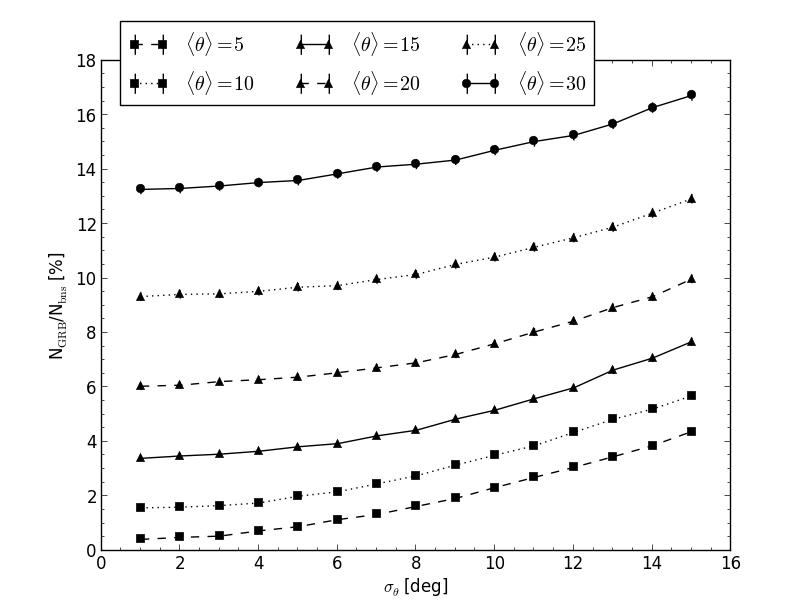
\includegraphics[width=15cm]{theta_dist_grbfrac.png}
    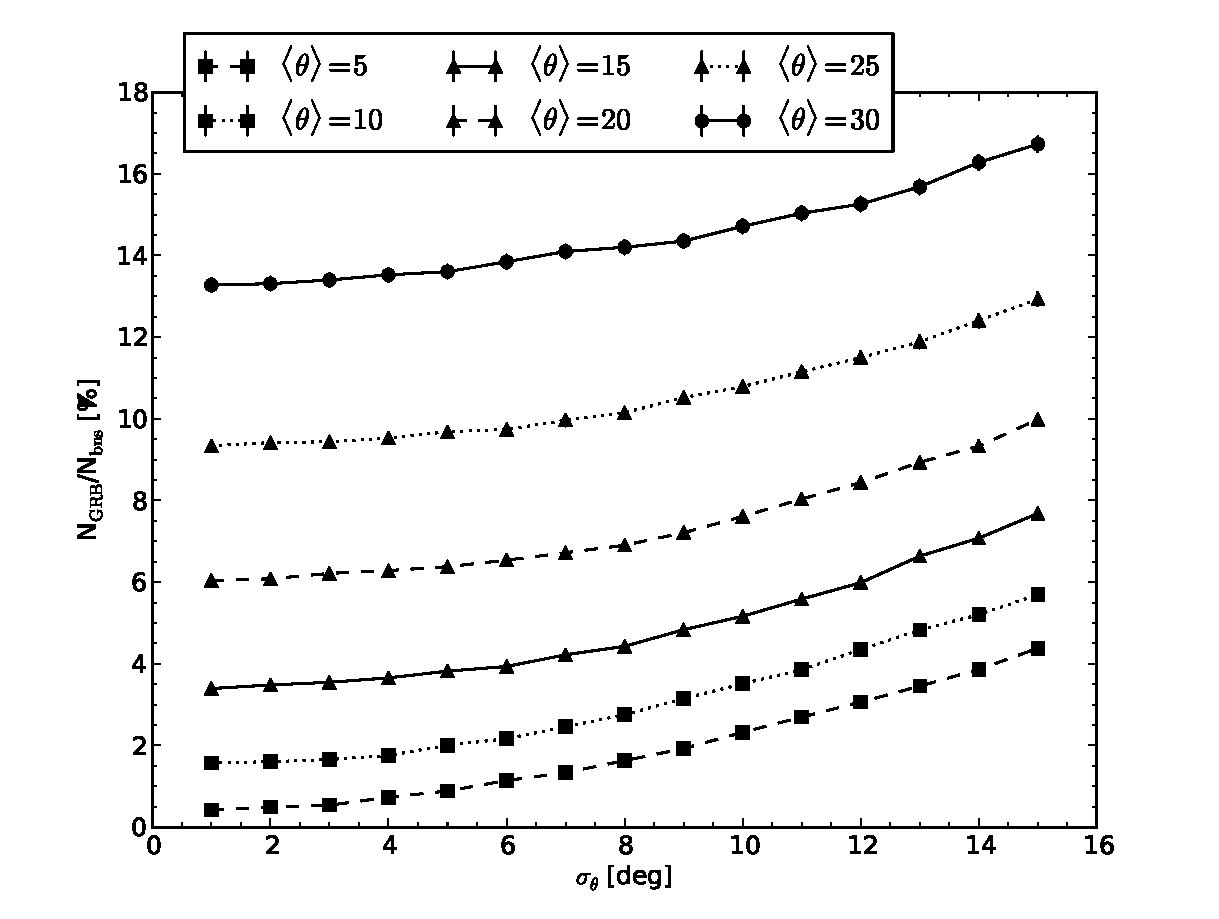
\includegraphics[width=0.5\linewidth]{theta_dist_grbfrac.pdf}
    \captionof{figure}{\label{fig:thetapopulation} Expected relative
    numbers of observed GRBs and binary coalescences for different distributions
on the GRB beaming angle.  Lines in the figure correspond to jet angle
population means, while the $x$-axis shows the width of the distribution.  All
distributions are Gaussian, truncated at $(0, 90]$ degrees.}
\end{center}\vspace{1cm}

\begin{comment}
    \begin{enumerate}
        \item Generate a population of binary inclination angles drawn from a
            uniform distribution in $\cos \iota$.  Call the size of this population
            $N_{\rm bns}$.
        \item For each of these `merger events' draw a GRB jet angle from a
            truncated Normal distribution with $N(\langle \theta \rangle,
            \sigma_{\theta})$.  If the inclination lies within the jet cone
            represented by this GRB jet angle, increment the number of `observed
            GRBs' $N_{\rm GRB}$ by 1.
        \item Study the ratio of observed GRBs to all mergers, $N_{\rm bns}/N_{\rm
            GRB}$ for a variety of jet angle distributions
    \end{enumerate}
\end{comment}

Figure~\ref{fig:thetapopulation} shows that the relative numbers of observed GRBs
to all binary mergers, for a given distribution mean, is quite insensitive to
the distribution width - the relative numbers only change by a few \%.
%
Note, however, that the relative numbers of events are degenerate across a range
of distribution means (e.g., the result for $p(\theta) = N(5,10)$ is
approximately the same as the result for $p(\theta) = N(10,5)$).  

{\bf Key finding}: event rate-based inferences on $\theta$ are really \emph{upper
bounds} on the \emph{mean} of the GRB jet angle population.

% What IS theta??

%\begin{wrapfigure}{r}{0.45\linewidth} 
%    \centering
%        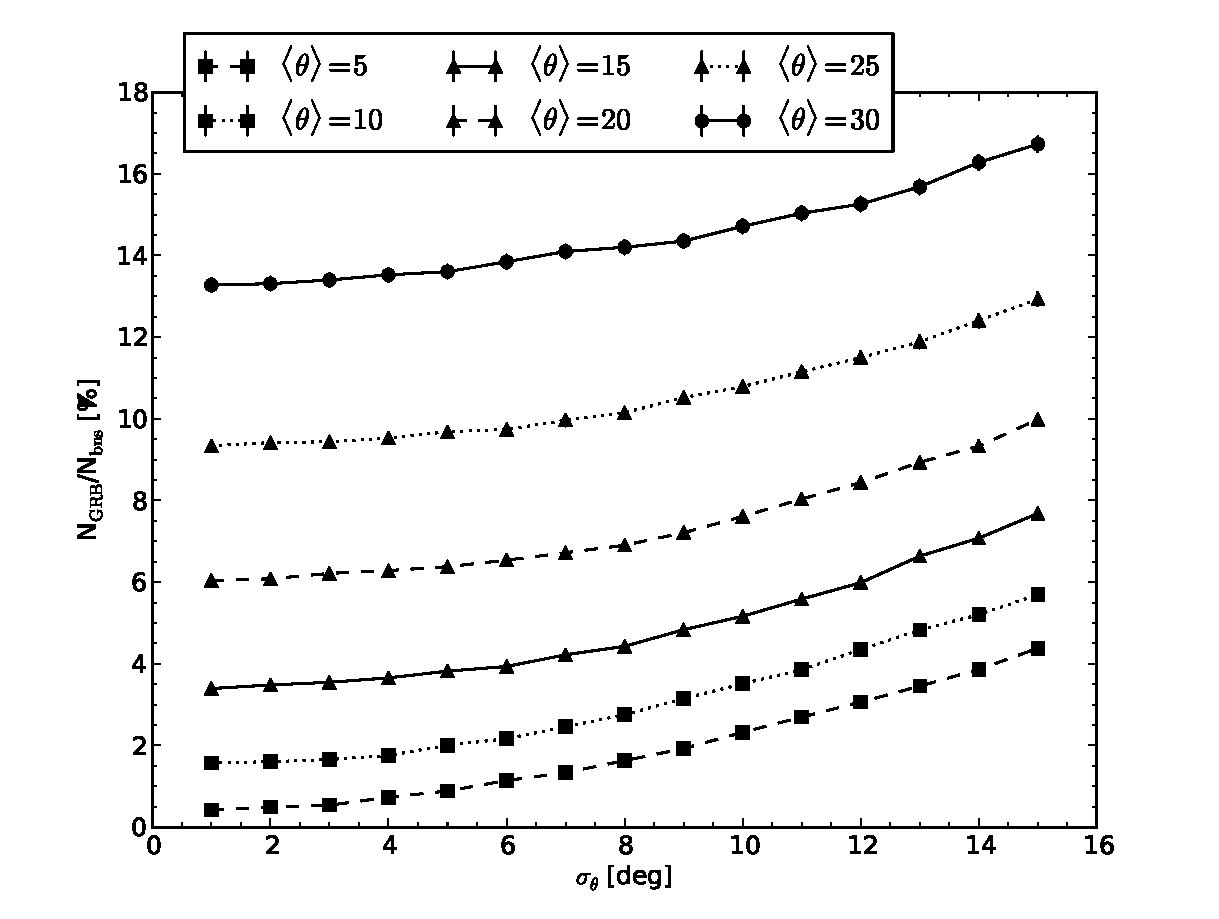
\includegraphics[width=15cm]{theta_dist_grbfrac.pdf}
        %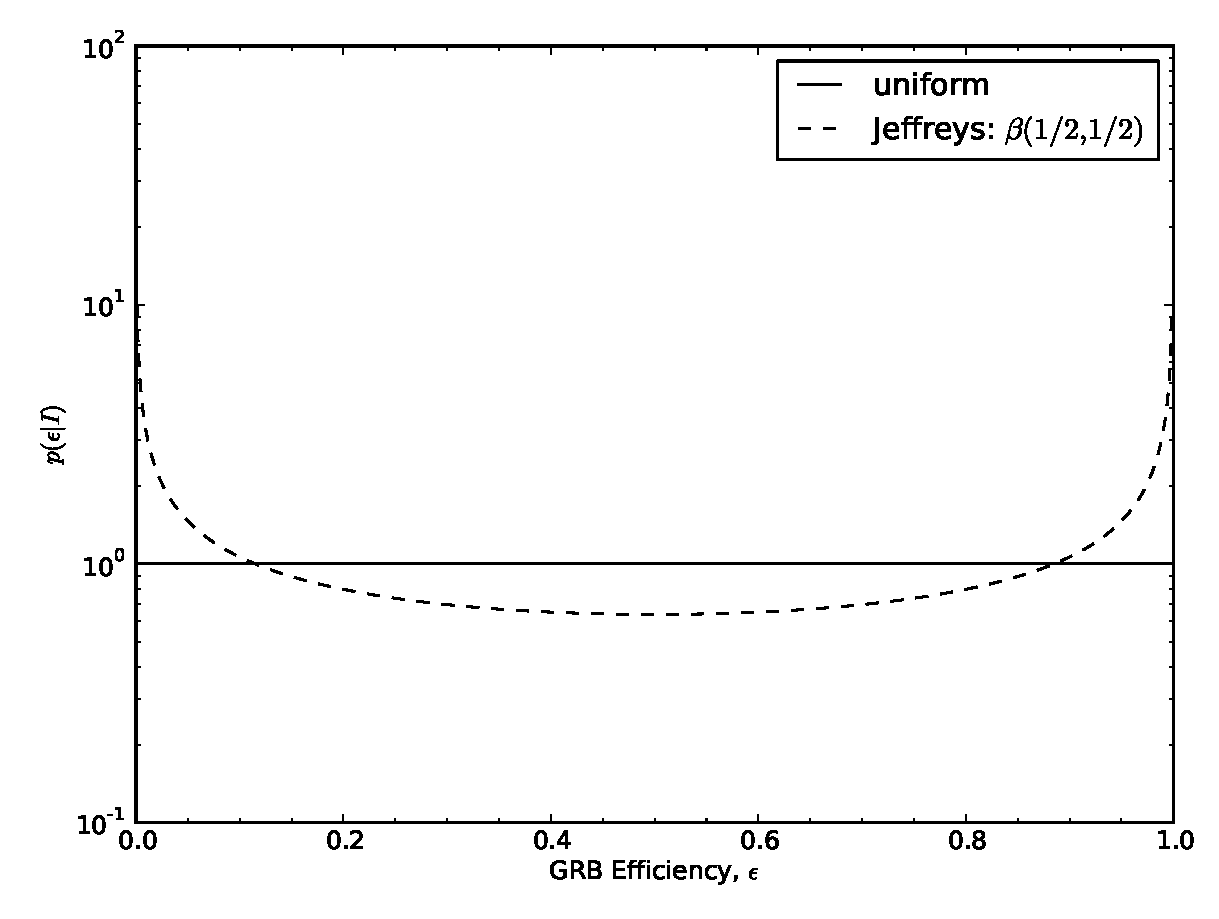
\includegraphics[width=0.5\linewidth]{efficiency_prior.pdf}
%        \captionof{figure}{Figure caption}
%\end{wrapfigure}

\section*{\centering Posterior Inferences On The Jet Angle}
%\To make meaningful inferences regarding the  mean GRB jet angle $\theta$ one
%must construct the posterior probability density function $p(\theta|D,I)$, where
%$D$ represents some data or measurement and $I$ some prior conditioning
%information.

%Given equation~\ref{eq:rate2theta}, a posterior PDF on the rate $\cbcrate$ and
%some prior information regarding the efficiency $\epsilon$ and the observed GRB
%rate $\grbrate$, one may construct a jet angle posterior via 
%transformation of the rate posterior:
Given equation~\ref{eq:rate2theta} one may construct a jet angle posterior via 
transformation of the rate posterior:
\begin{enumerate}
    \item Construct the joint-PDF on the jet angle $\theta$ and efficiency
        $\epsilon$ from the joint-PDF on the rate and the efficiency,

    \begin{equation}
    p(\theta,\epsilon) = p(\cbcrate,\epsilon)
    \left\lvert\left\lvert
    \frac{\partial(\cbcrate,\epsilon)}{\partial(\theta,\epsilon)}
    \right\rvert\right\rvert,
    \end{equation}

    where the second term is the Jacobian determinant for the transformation and
    we assume that the rate posterior and the prior PDF on the efficiency are
    logically independent, such that:
    %
    %\begin{equation}
        $p(\cbcrate, \epsilon) =  p(\epsilon|\cbcrate)p(\cbcrate) =
        p(\epsilon)p(\cbcrate)$
    %\end{equation}

    \item Inferences on the jet angle are then arrived at by marginalising the joint
        posterior $p(\theta,\epsilon)$ over the unknown efficency:

        \begin{eqnarray}
        p(\theta) = \int_{\epsilon} p(\theta,\epsilon)~\diff \epsilon =
        \int_{\epsilon} ~\diff \epsilon p(\cbcrate)(\epsilon)
            \left\lvert\left\lvert
            \frac{\partial(\cbcrate,\epsilon)}{\partial(\theta,\epsilon)}
            \right\rvert\right\rvert,
        \end{eqnarray}

\end{enumerate}

Our approach requires the explicit specification of a prior probability
distribution function for the GRB efficiency $\epsilon$ (effectively, the
average probability that any given binary merger yields a \grb{} counterpart).
For the purposes of this study, we consider:
\begin{itemize}
    \item $p(\epsilon|I) = \delta(\epsilon-1.0)$: Efficiency known; all mergers
        yield \grb{s}
    \item $p(\epsilon|I) = \delta(\epsilon-0.5)$: Efficiency known; 50\% of
        mergers yield \grb{s}
    \item $p(\epsilon|I) = U(0,1])$: Unknown efficiency, equal probability in
        $(0,1]$
    \item $p(\epsilon|I) = \beta(0,1])$: Unknown efficiency, Jeffrey's prior for
        Bernoulli trial (success=\grb{}!)
\end{itemize}

%%%%%%%%%%%%%%%%%%%%%%%%%%%%%%%%%55
\begin{comment}
where the Jacobian matrix is given by,
% Increase matrix line spacing
\begingroup
\renewcommand*{\arraystretch}{1.5}

% matrix:
\begin{equation}
\frac{\partial (\cbcrate,\epsilon)}{\partial(\theta,\epsilon)} =
\begin{bmatrix}
\frac{\partial \cbcrate}{\partial \theta} & \frac{\partial \cbcrate}{\partial \epsilon} \\
\frac{\partial \epsilon}{\partial \theta} & \frac{\partial \epsilon}{\partial \epsilon}
\end{bmatrix}.
\end{equation}

% end line spacing increase
\endgroup
\end{comment}
%%%%%%%%%%%%%%%%%%%%%%%%%%%%%%%%%55

%------------------------------------------------
%------------------------------------------------
% Efficiency Prior
\begin{comment}
\subsection*{Prior on GRB Efficiency, $\epsilon$}

Sed fringilla tempus hendrerit. Vestibulum ante ipsum primis in faucibus orci
luctus et ultrices posuere cubilia Curae; Etiam ut elit sit amet metus lobortis
consequat sit amet in libero. Lorem ipsum dolor sit amet, consectetur adipiscing
elit. Phasellus vel sem magna. Nunc at convallis urna. isus ante. Pellentesque

%\begin{wrapfigure}{r}{0.45\linewidth} 
%    \centering
%        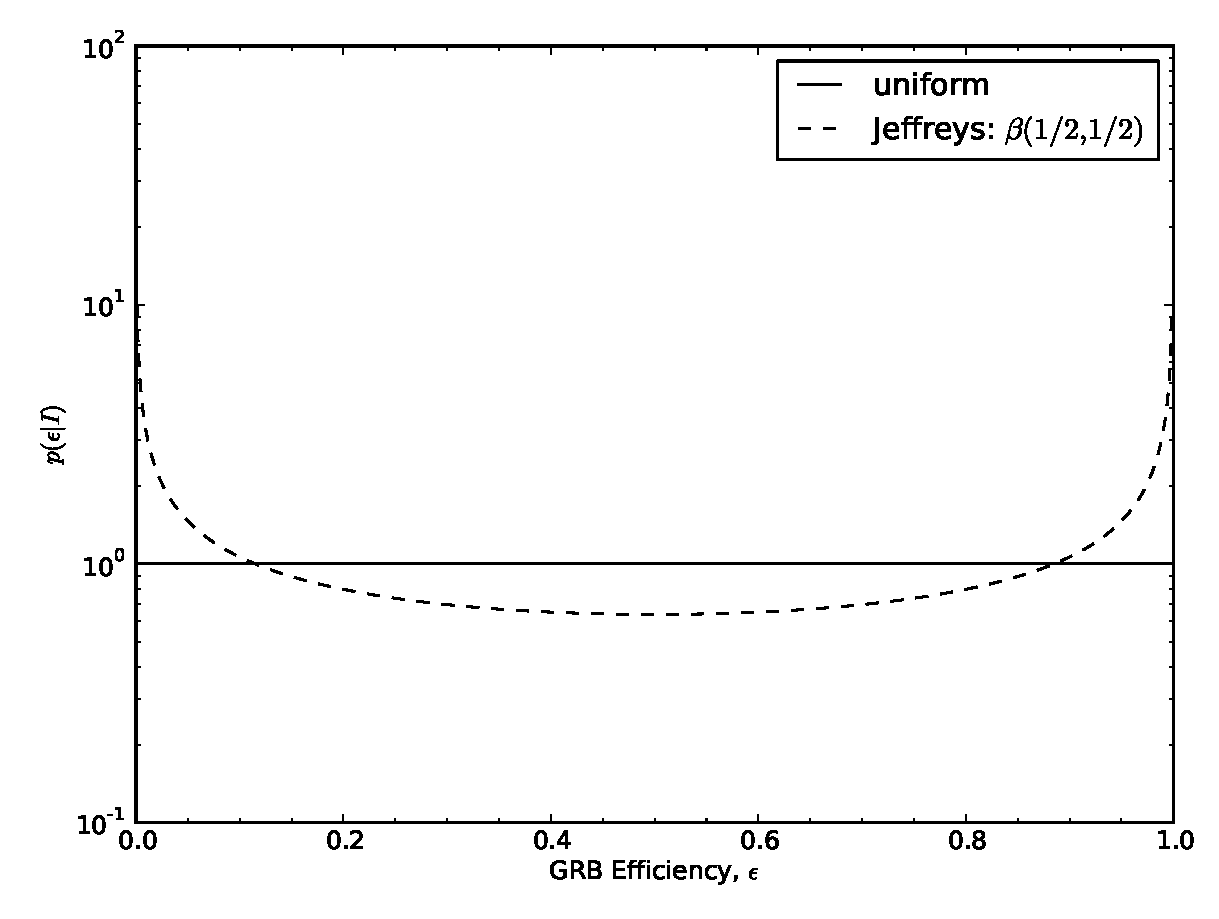
\includegraphics[width=15cm]{efficiency_prior.pdf}
%        %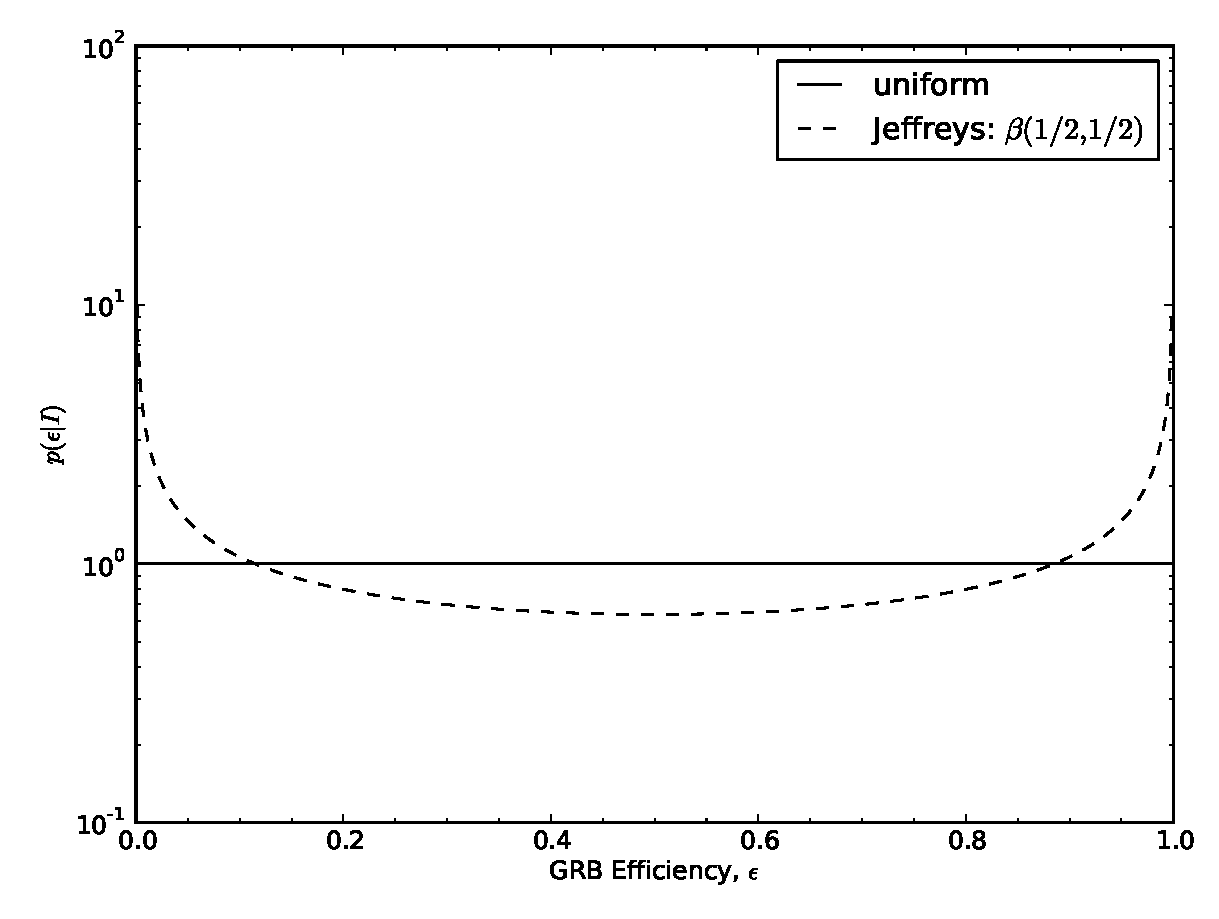
\includegraphics[width=0.5\linewidth]{efficiency_prior.pdf}
%        \captionof{figure}{Figure caption}
%\end{wrapfigure}
\begin{center}\vspace{1cm}
        %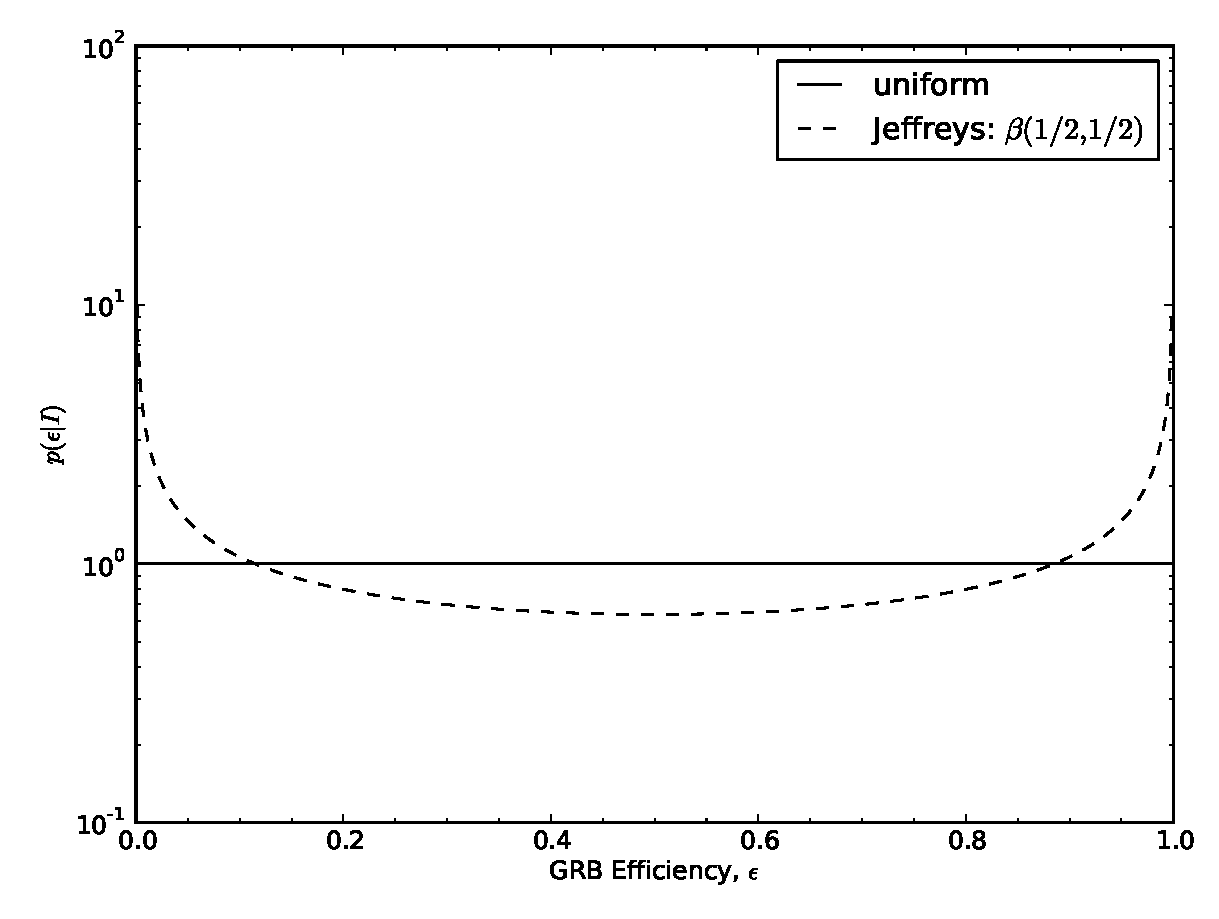
\includegraphics[width=15cm]{efficiency_prior.pdf}
        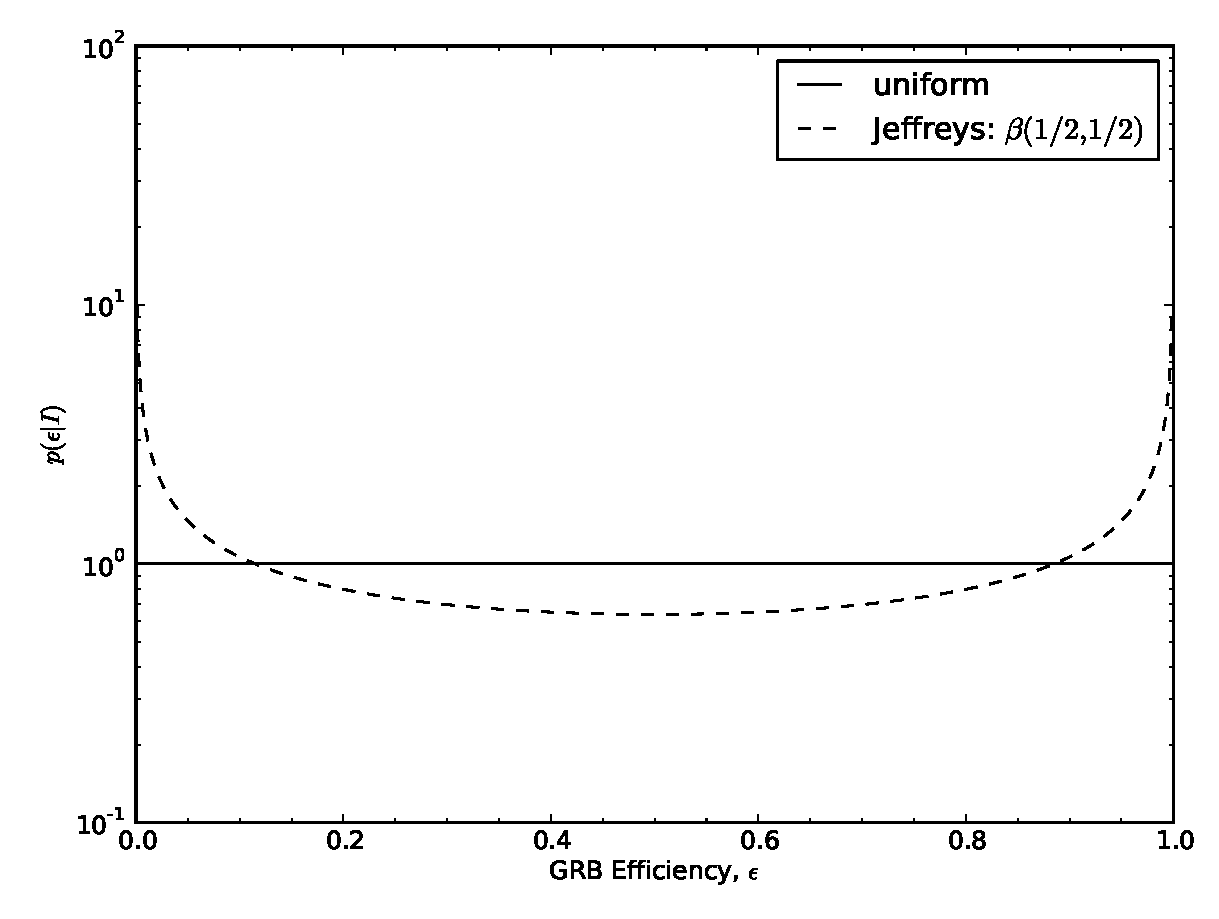
\includegraphics[width=0.48\linewidth]{efficiency_prior.pdf}
        \captionof{figure}{Figure caption}
\end{center}\vspace{1cm}

Sed fringilla tempus hendrerit. Vestibulum ante ipsum primis in faucibus orci
luctus et ultrices posuere cubilia Curae; Etiam ut elit sit amet metus lobortis
consequat sit amet in libero. Lorem ipsum dolor sit amet, consectetur adipiscing
elit. Phasellus vel sem magna. Nunc at convallis urna. isus ante. Pellentesque
condimentum dui. Etiam sagittis purus non tellus tempor volutpat. Donec et dui
non massa tristique adipiscing. Quisque vestibulum eros eu. Phasellus imperdiet,
tortor vitae congue bibendum, felis enim sagittis lorem, et volutpat ante orci
sagittis mi. Morbi rutrum laoreet semper. Morbi accumsan enim nec tortor
consectetur non commodo nisi sollicitudin. Proin sollicitudin. Pellentesque eget
orci eros. Fusce ultricies, tellus et pellentesque fringilla, ante massa luctus
libero, quis tristique purus urna nec nibh.
\end{comment}


%----------------------------------------------------------------------------------------
%	iLIGO
%----------------------------------------------------------------------------------------
\section*{\centering Constraints From The Initial Detector Era}


%\subsection*{Constructing The Rate Posterior}
%\begin{equation}\label{eq:loudestEventPosterior}
%p(\cbcrate | C_L({\rhostar}), T, \Lambda) \propto p(\cbcrate) \left[ \frac{1+\Lambda
%C_L(\rhostar) T}{1+\Lambda}\right] e^{-\cbcrate C_L(\rhostar) T}
%\end{equation}


%\subsection*{Results}


  \begin{minipage}{\columnwidth}
    \makeatletter
    \newcommand{\@captype}{figure}
    \makeatother
    \centering
    \subfloat[Rate Posterior]{%
      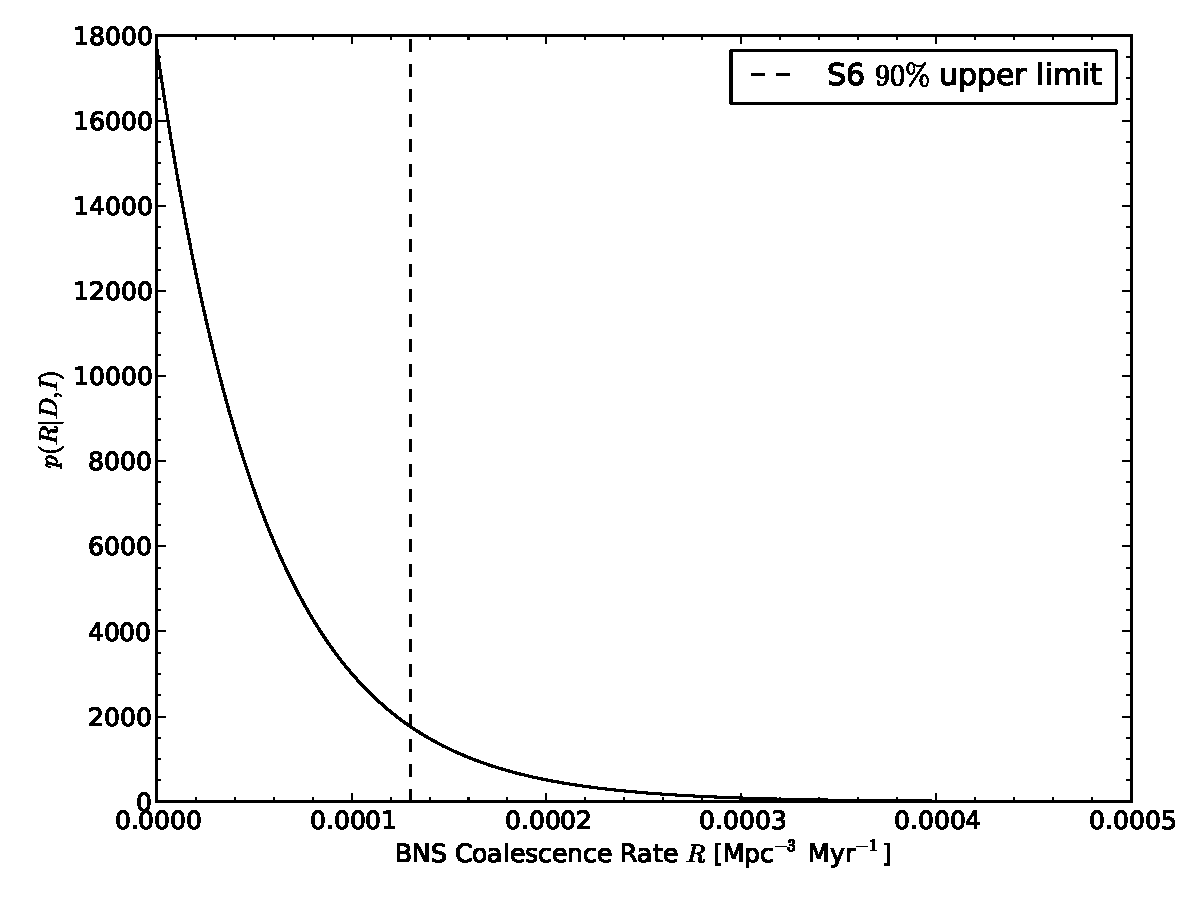
\includegraphics[width=0.45\linewidth]{S6_rate.pdf}%
      \label{fig:}%
    }\qquad%
    \subfloat[Jet Posterior]{%
      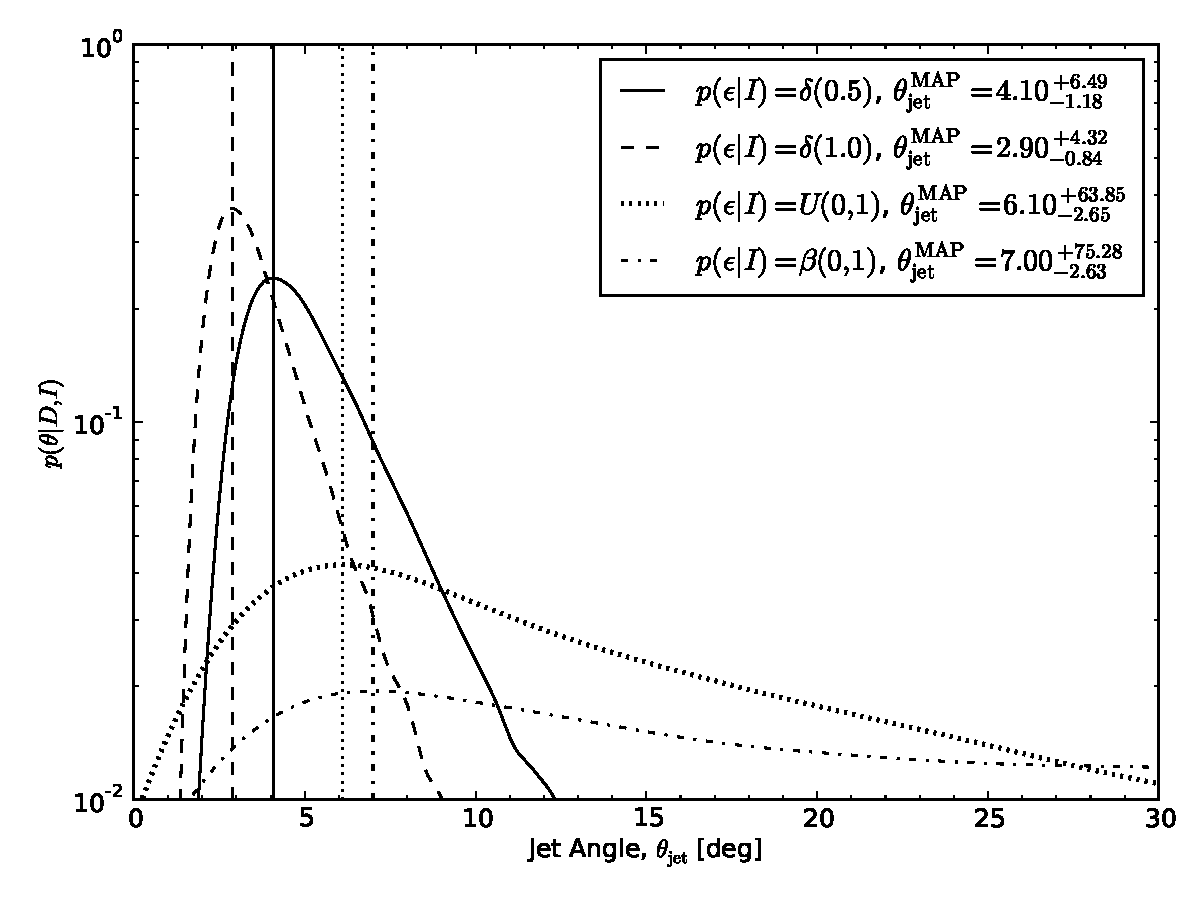
\includegraphics[width=0.45\linewidth]{jet_angle_posterior_iligo.pdf}%
      \label{fig:}%
    }
    \caption{S6 results}
  \end{minipage}

%----------------------------------------------------------------------------------------
%	aLIGO
%----------------------------------------------------------------------------------------
\section*{\centering Constraints In The Advanced Detector Era}

%\subsection*{Constructing The Rate Posterior}

\begin{comment}
    So let $b=10^{-2}$\,yr$^{-1}$.  From there, we can get the detection rate
    posterior using equations 14.10--14.12 of Gregory.  The measured rate $r$
    consists of two components, one due to a signal of interest, $s$, and the other
    a known background rate, $b$:
    \begin{equation}
    r = s + b
    \begin{cases}
    s = \text{signal rate} \\
    b = \text{background rate}
    \end{cases}
    \end{equation}
    %
    Since the background rate is known,
    \begin{equation}
    p(s|n,b,I) = p(r|n,b,I),
    \end{equation}
    %
    where $n$ is the number of \gw{} detections.  From eq 14.8 of Gregory, we get
    to:
    \begin{equation}
    p(s|n,b,I) = C \frac{ T\left[(s+b)T\right]^n e^{-(s+b)T}}{n!},
    \end{equation}
    %
    where,
    \begin{eqnarray}
    C^{-1} & = &\frac{e^{-bT}}{n!} \int_0^{\infty}\diff(sT)(s+b)^n T^n e^{-sT}\\
    & = & \sum_{i=0}^n \frac{ (bT)^i e^{-bT}}{i!}.
    \end{eqnarray}

    In particular,  the detection rate for a given type of binary coalescence in
    LIGO-Virgo is given by equation\,1 in~\cite{rates_paper},
    \begin{equation}
    %\dot{N} = \cbcrate \times N_G,
    s = \cbcrate \times N_G,
    \end{equation}
    %
    where $\cbcrate$ is the coalescence rate of that type of binary per galaxy and
    $N_G$ is the number of galaxies accessible with a search for the relevant binary
    type.  $N_G$ is well approximated at large distances by,
    %
    \begin{equation}
    N_G = \frac{4}{3} \pi \left( \frac{D_{\textrm{horizon}}}{\textrm{Mpc}}
    \right)^3 (2.26)^{-3} (0.0116).
    \end{equation}
    %
    The reader is directed to~\cite{rates_paper} for a discussion of the numerical
    factors in the equation above.

    Finally, we recognise that $\dot{N}$ is the signal rate $s$ in
    equation~\ref{eq:signal_rate_posterior} so that we arrive at the desired
    posterior on the binary coalescence rate, 
    %
    \begin{eqnarray}
    p(\cbcrate|N_{\textrm{det}},I) & = & p(s|N_{\textrm{det}},I) \left|\frac{\diff
    s}{\diff \cbcrate}\right| \\
    & = & N_G . p(s|N_{\textrm{det}},I)
    \end{eqnarray}

\end{comment}

\subsection*{Validation}

\begin{center}\vspace{1cm}
    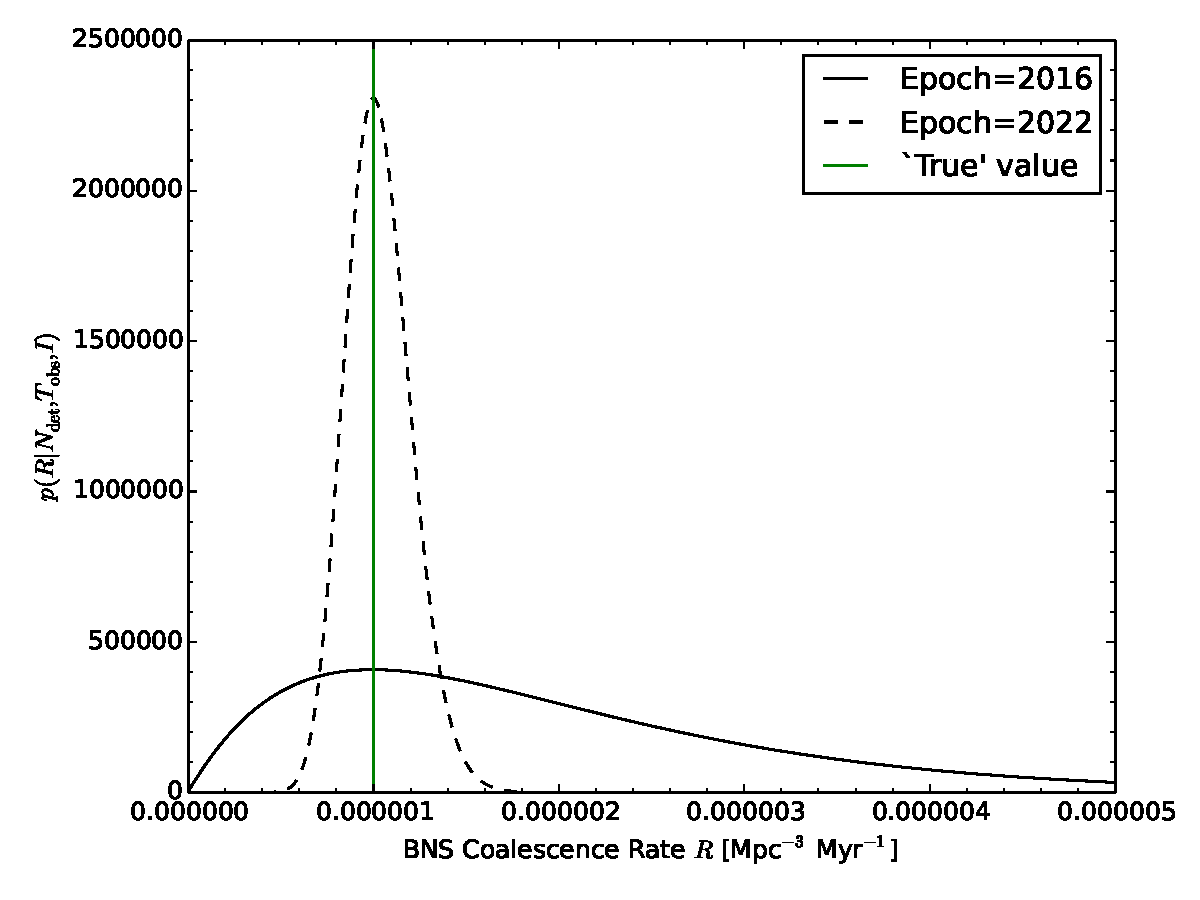
\includegraphics[width=0.5\linewidth]{aligo_rate_re.pdf}
    \captionof{figure}{Figure caption}
\end{center}\vspace{1cm}

\begin{minipage}{\columnwidth}
  \makeatletter
  \newcommand{\@captype}{figure}
  \makeatother
  \centering
  \subfloat[Rate Posterior]{%
    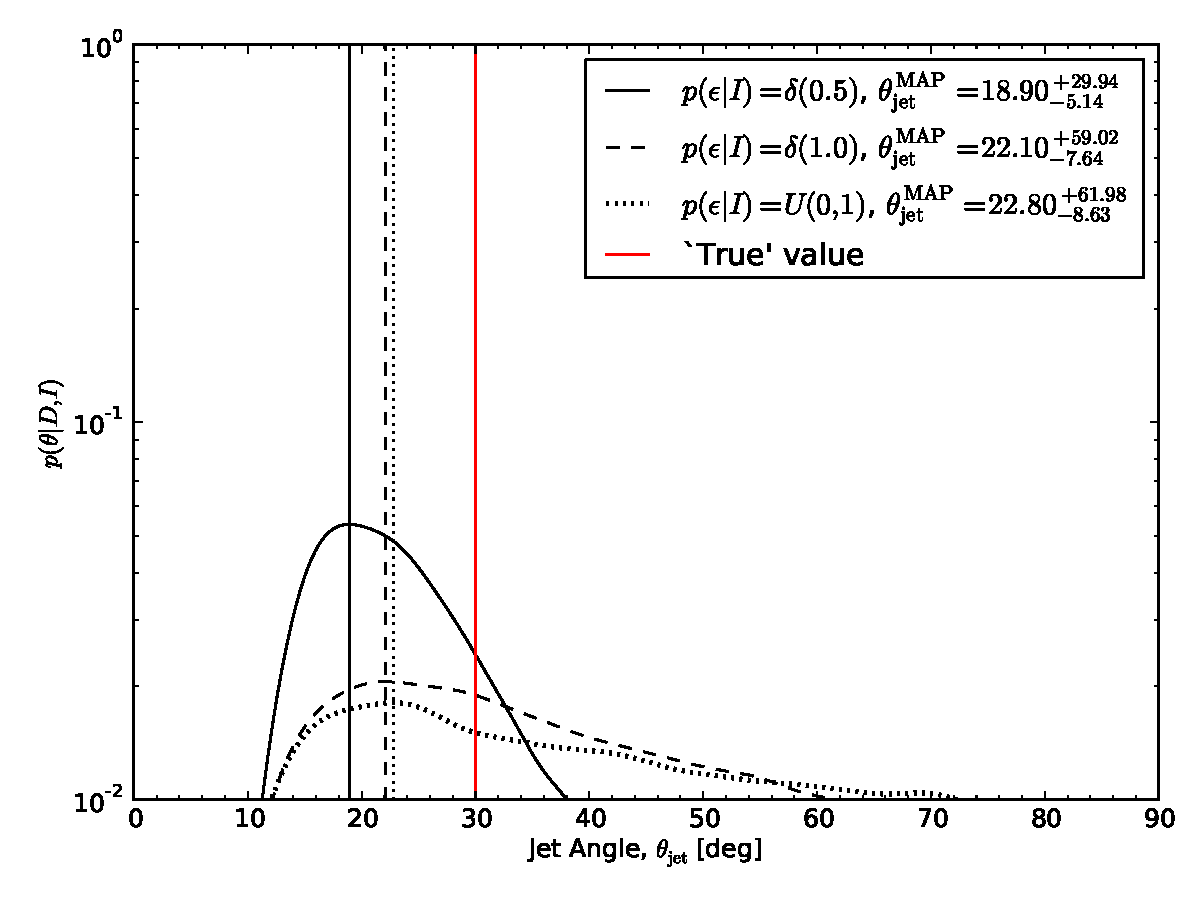
\includegraphics[width=0.45\linewidth]{jet_angle_posterior_aligo_2016.pdf}%
    \label{fig:}%
  }\qquad%
  \subfloat[Jet Posterior]{%
    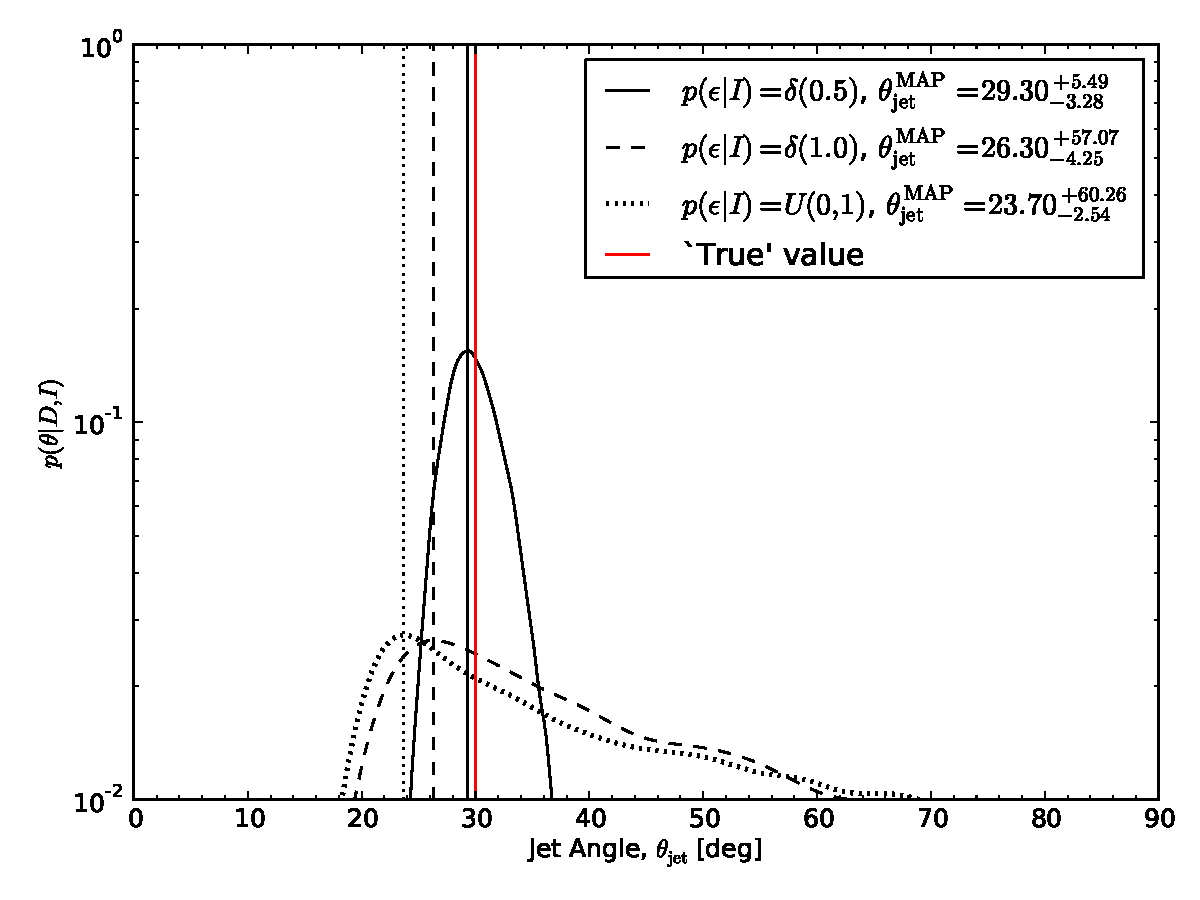
\includegraphics[width=0.45\linewidth]{jet_angle_posterior_aligo_2022.pdf}%
    \label{fig:}%
  }
  \caption{Example results for $\theta_{\rm jet}=30^{\circ}$ and binary
  coalescence rates in~\cite{scenarios} to derive a `simulated' GRB rate.}
\end{minipage}

\subsection*{Predictions}

\begin{minipage}{\columnwidth}
  \makeatletter
  \newcommand{\@captype}{figure}
  \makeatother
  \centering
  \subfloat[Rate Posterior]{%
    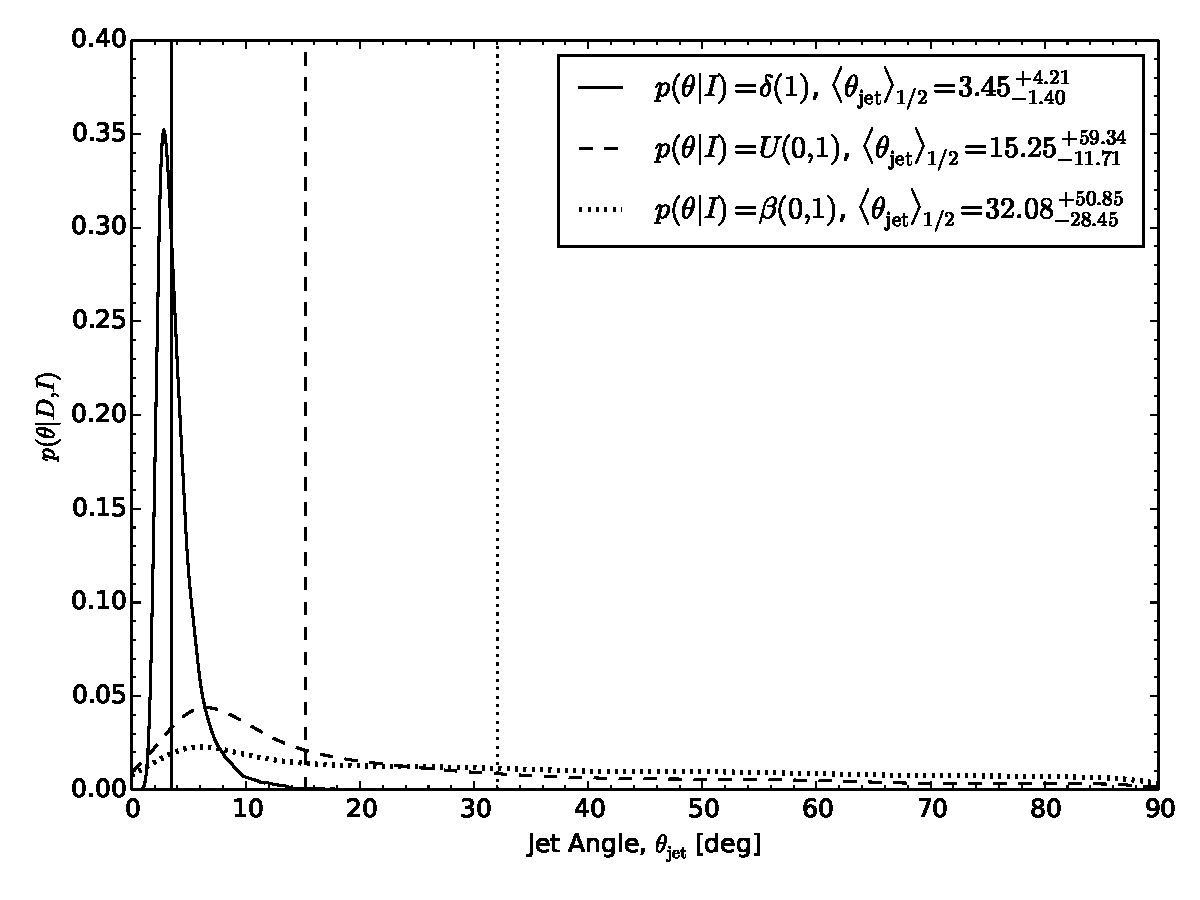
\includegraphics[width=0.45\linewidth]{jet_angle_posterior_aligo_2016_real.pdf}%
    \label{fig:}%
  }\qquad%
  \subfloat[Jet Posterior]{%
    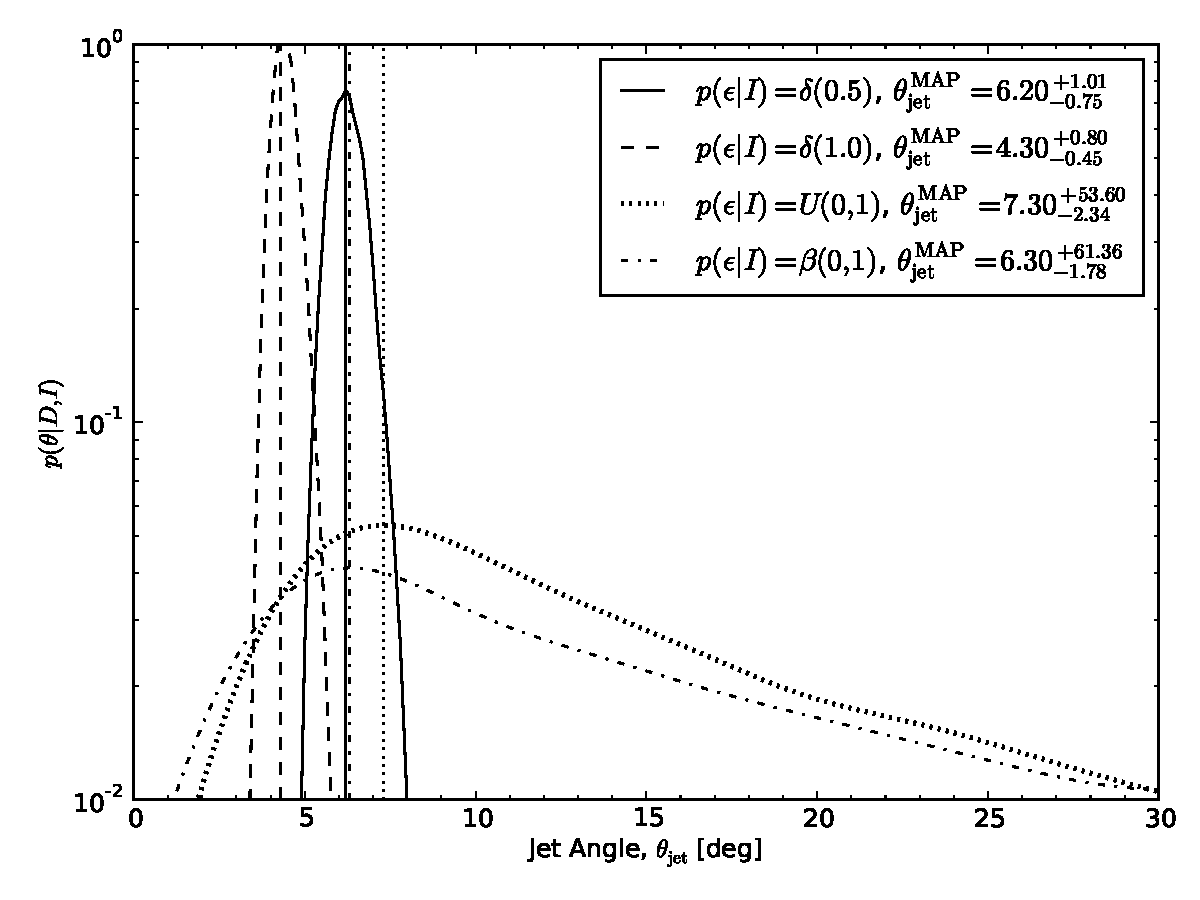
\includegraphics[width=0.45\linewidth]{jet_angle_posterior_aligo_2022_real.pdf}%
    \label{fig:}%
  }
  \caption{Results in ADE assuming $\grbrate =
      3\times10^{-9}$\,Mpc$^{-3}$yr$^{-1}$ and binary coalescence rates
  in~\cite{scenarios}.}
\end{minipage}

%----------------------------------------------------------------------------------------
%	CONCLUSIONS
%----------------------------------------------------------------------------------------

\color{SaddleBrown} % SaddleBrown color for the conclusions to make them stand out

\section*{Conclusions}

\begin{itemize}
\item Pellentesque eget orci eros. Fusce ultricies, tellus et pellentesque fringilla, ante massa luctus libero, quis tristique purus urna nec nibh. Phasellus fermentum rutrum elementum. Nam quis justo lectus.
\item Vestibulum sem ante, hendrerit a gravida ac, blandit quis magna.
\item Donec sem metus, facilisis at condimentum eget, vehicula ut massa. Morbi consequat, diam sed convallis tincidunt, arcu nunc.
\item Nunc at convallis urna. isus ante. Pellentesque condimentum dui. Etiam sagittis purus non tellus tempor volutpat. Donec et dui non massa tristique adipiscing.
\end{itemize}

\color{DarkSlateGray} % Set the color back to DarkSlateGray for the rest of the content


 %----------------------------------------------------------------------------------------
%	REFERENCES
%----------------------------------------------------------------------------------------

\nocite{*} % Print all references regardless of whether they were cited in the poster or not
\bibliographystyle{plain} % Plain referencing style
\bibliography{sample} % Use the example bibliography file sample.bib

%----------------------------------------------------------------------------------------
%	ACKNOWLEDGEMENTS
%----------------------------------------------------------------------------------------

%\section*{Acknowledgements}

%Etiam fermentum, arcu ut gravida fringilla, dolor arcu laoreet justo, ut
%imperdiet urna arcu a arcu. Donec nec ante a dui tempus consectetur. Cras nisi
%turpis, dapibus sit amet mattis sed, laoreet.

%----------------------------------------------------------------------------------------

\end{multicols}
\end{document}
